\documentclass[a4paper,12pt]{article}
\usepackage{listings}
\usepackage{amsmath}
\usepackage{amssymb}
\usepackage{graphicx}

\author{E. Routledge}
\date{01 Nov 2022}
\title{Sudoku and Other Related Problems}

\begin{document}
\lstset{language=Python}
\maketitle

% ~~~~~~~~~~~~~~~~~~~~~~~~~~~~~~~~~~~~~~~~~~~~~~~~~~~~~~~~~~~~~~~~~~~~~~~~~~~~~~~~~~~~~~~~~~~~ %
\section{Introduction}
		Sudoku is a simple logic game, in the standard $9 \times 9$ (or $3 \times 3 \times 3 \times 3$) 
		one must complete the grid such that every row, column and box contains the numbers 1 to 9, that is all. 
		Yet it leads to interesting and difficult puzzles.
	\subsection{History}
% ~~~~~~~~~~~~~~~~~~~~~~~~~~~~~~~~~~~~~~~~~~~~~~~~~~~~~~~~~~~~~~~~~~~~~~~~~~~~~~~~~~~~~~~~~~~~ %
\section{Sudoku is Hard}

		Sudoku can be described in a single rule but it is in fact a hard problem to solve.
		Instances of the puzzle requiring complex x wing and y wing strategies are not what makes the puzzle hard to solve,
		it is hardness through a provable, computational lense for which this section cares. 
		
	\subsection{Computational Complexity an Introduction}
		\textbf{What is NP completeness?}
		We care about decision problems, these are problems that given an input  produce a 'yes' or 'no' answer. We care about three of the subsets of these problems: P is the the class of problems that can be solved in polynomial time by a Turing machine; NP is the class of problems that can be verified in polynomial time and solved in polynomial time by a non-deterministic Turing machine, finally, the NP-complete set has problems that any NP problem can be reduced to in polynomial time (if there is a NP-complete problem that can be solved in polynomial time then P=NP, this is one of the millenium prize problems).
		This is to say NP problems are hard, it is assumed they cannot be solved in polynomial time ($P \neq NP$) and are therefore infeesible for large inputs.

\begin{figure}[h!]
	\begin{center}
		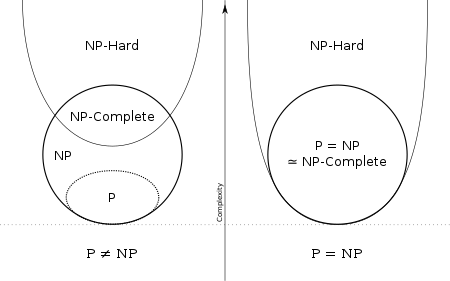
\includegraphics[width=60mm]{P_np.svg}
	\end{center}
	\caption{P, NP, NP-complete \& NP-hard sets \cite{P_NP_Figure}}
\end{figure}

		\textbf{How to prove NP completeness generally?}
		Show verifier has a polynomial or less runtime.
		Reduce a known NP-complete problem to the problem you wish to prove is NP-complete (call this $x$), one does this by transforming the input of a known NP-complete problem to the input $x$. This proves that the $x$ is at least as hard as the NP-complete problem as if we had access to an polynomial time algorithm to solve $x$ we could solve the known NP-complete problem in polynomial time too creating a contradiction.

\textbf{Our base NP-complete problem.} If, as the above suggests, we require a NP-complete problem to prove a problem is NP-complete then we seem to have reached a paradox. Luckily we have the Cook-Levin Theorem.

\textit{Cook-Levin Theorem:} SAT is NP-Complete
	
\textit{Proof:} cite 

\textit{Definition: } SAT is the following decision problem. Given a set of boolean variables $B$ and a collection of clauses $C$ does a valid truth assignment exist that satisfies $C$?

We now have a NP-complete problem to reduce other problems to.

	\subsection{Validation is Easy}
Valid Grid decision problem:

		\begin{equation}
			\Psi(\text{grid}(n^2,n^2)) = \begin{cases}	
							     \text{True if the grid is valid} \\
							     \text{False if the grid is invalid}.
							     \end{cases}
		\end{equation}

There exists an algorithm to do this in polynomial time with respect to the dimensions of the grid. 
\begin{enumerate}
\item For each row in the grid check there exists no repeated numbers. $O(n^2)$
\item For each column in the grid check there exists no repeated numbers. $O(n^2)$
\item For each box in the grid check there exists no repeated numbers. $O(n^2)$
\end{enumerate}
If all tests pass return True else return False.
This algorithm has complexity of $O(n^2 + n^2 + n^2) = O(3n^2) = O(n^2)$, this is polynomial and therefore $\Psi(\text{grid}) \in P$.

	\subsection{Finding a Solution is Hard}
		
Finding a solution to sudoku is NP-complete, let us define the decision problem:

		\begin{equation}
		        \Phi (\text{grid}(n^2,n^2)) = \begin{cases}
		            \text{True if a solution exists} \\
		            \text{False if a solution does not exist}.
				\end{cases}
		\end{equation}

Our question now is does there exist a function $\Phi$ that when given an instance of the problem (in this case a grid of numbers and blanks) will, in polynomial time or less return True if it can be solved and False otherwise.

\textbf{\underline{Proof}}

The \textbf{verifier} is $O(n^2)$, as will be seen in the above subsection 'Validation is Easy'.

Now we need a \textbf{reduction} from sudoku to a known NP-complete problem to prove sudoku is at least as hard. We will be creating a chain of reductions: Sudoku $\geq_p$  Latin Square $\geq_p$  Triangulated Tripartite $\geq_p$  3SAT and then prove 3SAT is NP-complete.

\textbf{Sudoku $\geq_p$ Latin Square}

\textit{What is the Latin Square decision problem?} Given a partially filled $n \times n$ grid, can the empty squares be filled in such that the grid satisfies the latin square properties (each row and column has values 1 to n exactly)?

To reduce a given sudoku grid of size $n^2 \times n^2$ to a latin square (definition of which see in Other Related Problems - Latin Squares) take the first row of boxes and select the first column from each box, these will make a $n \times n$ latin square. If any numbers are repeated we can relabel without a problem 

\textbf{Latin Square $\geq_p$ Triangulated Tripartite}

\textbf{Triangulated Tripartite $\geq_p$ 3SAT}

\textbf{3SAT is NP-Complete}

\textit{What is 3SAT?} With a set of boolean variables $B$ and a collection of clauses $C$, with at most 3 literals (a literal is any $b \in B$ or its negation $\bar{b}$) in each, does a valid truth assignment exist that satisfies $C$?
		\begin{equation}
		        \phi (C,B) = \begin{cases}
		            \text{True if a truth assignment exists} \\
		            \text{False if a truth assignment does not exist}.
				\end{cases}
		\end{equation}
This decision problem is therefore an enforced limitation of SAT as defined in the subsection Computational Complexity an Introduction.

		\textit{Proof}
Given a truth assignment $t$ check each clause is satisfied, if all are satisfied return True else False, this algorithm is at most the length of $C$ multiplied by the length of $B$. $O(BC)$ is polynomial, a polynomial verifier exists. 

Given a SAT instance with the input sets of $B$ and $C$. $C$ is in conjunctive normal form (every clause set can be converted to an equivalent set in CNF form \cite{CNF}) such that $\forall c \in C$ and for some $b_1, ... ,b_n \in B$, $c = b_1 \lor b_2 \lor ... \lor b_n$. For each $c \in C$ with more than 3 literals we can transform these to a new set of clauses of length 3. 

For $c = b_1 \lor b_2 \lor ... \lor b_n$ we introduce a new literal: $a_1$ to give $b_1 \lor b_2 \lor a_1$, $\bar{b_1} \lor a_1$, $\bar{b_2} \lor a_1$ and $a_1 \lor b_3 \lor ... \lor b_n$. Then $a_1 \lor b_3 \lor ... \lor b_n$ becomes $b_3 \lor b_4 \lor a_2$, $\bar{b_3} \lor a_2$, $\bar{b_4} \lor a_2$ and $a_1 \lor a_2 \lor b_5 \lor ... \lor b_n$. This continues at most $n/2$ times to give $a_1 \lor ... \lor a_{n/2}$ or $a_1 \lor ... \lor a_{n/2} \lor b_n$ if n is odd. 

Because we can convert a clause larger than 3 into multiple clauses of at most 3 literals in linear time ($O(n/2 + n/4 + ...) = O(n)$) this means we can reduce SAT to 3SAT in polynomial time. 

As SAT is NP-complete by the Cook-Levin Theorem, this proves 3SAT is NP-Complete. $\square$
		
Alternative reduction Sudoku $\geq_p$  $n^2$ Graph Colouring.

	\subsection{Determining Uniqueness is Hard}

It is hard to determine if a puzzle has a unique solution?
		
% ~~~~~~~~~~~~~~~~~~~~~~~~~~~~~~~~~~~~~~~~~~~~~~~~~~~~~~~~~~~~~~~~~~~~~~~~~~~~~~~~~~~~~~~~~~~~ %
\section{Other Related Problems}
	\subsection{Latin Squares}

		\begin{itemize}
		\item{A latin square is an n by n matrix filled with n characters that must not repeat along columns or rows.}
		\item{Reduced Form - f first row and column is in the natural order}
		\item{Equivalence classes}
		\item{Number of n by n latin squares is bounded}
		\item{Latin squares can be considered a bipartite graph}
		\item{Agronomic Research}
		\item{Latin hypercube}
		\end{itemize}

	\subsection{Magic Squares}

		\begin{itemize}
		\item{A magic square is a matrix of numbers with each column, row and diagonal summing to the same value, 
		this value is known as a magic constant and the degree is the number of columns/rows.}
		\item{A normal magic square is one containing the integers 1 to $n^2$.}
		\item{Magic Squares with repeating digits are considered trivial.}
		\item{Semimagic squares omit the diagnonal sums also summing to the magic constant.}

		\item{Truly thought to be magic Shams Al-ma'arif.}

		\item{Generation, there exists not completely general techniques. Diamond Method}

		\item{Associative Magic Squares}
		\item{Pandiagonal Magic Squares}
		\item{Most-Perfect Magic Squares}
		
		\item{Equivalence classes for $n<=5$ but not for higher orders.}
		\item{The enumeration of most perfect magic squares of any order.}

		\item{880 distinct magic squares of order four}

		\item{Normal magic squares can be constructed for all values except 2}
		\item{Preserving the magic property when transformed}

		\item{Methods of construction}

		\item{Multiplicative magic squares - produce infinite}

		\item{Sator square}

		\item{magic square of squares - Parker Square is a failed example of this}
		\end{itemize}
	
	\subsection{Greco-Latin Squares}

		\begin{itemize}
		\item{Two orthogonal latin squares super imposed, such that the pairs of values are unique.}
		\item{Group based greco latin squares}
		\item{Eulers interest came from construction of magic squares}
		\item{Exists for all but 2 and 6.}
		\end{itemize}

% ~~~~~~~~~~~~~~~~~~~~~~~~~~~~~~~~~~~~~~~~~~~~~~~~~~~~~~~~~~~~~~~~~~~~~~~~~~~~~~~~~~~~~~~~~~~~ %
\section{Solving Techniques}
	\subsection{Backtracking}
		
		The standard way to solve a $9 \times 9$ sudoku puzzle is by the backtracking algorithm. 
		This is a brute force method with a few optimisations.
		One can expect to find this algorithm in a computer science course introduction to recursion, that is to say it is not a complex concept 
		and while useful for the usual sizes, as soon as we increase to $16 \times 16$ this becomes infeesible.
		Multiplication tables of quasigroups.
		Orthogonal latin squares are used in error correcting codes.
		
		\begin{lstlisting}[caption=Backtracking]
def Backtracking(grid):
    for each row:
        for each column:
            if grid is empty at this potion:
                try a value in this position
                Backtracking(grid with new value)
                if successful:
                    return grid
                else:
                    try another value
                if no values left to try:
                    return False
    return grid						
		\end{lstlisting}
		
		Why does brute force not work for larger examples?

	\subsection{Stochastic Methods}
		\subsubsection{Simulated Annealing} 
		\subsubsection{Genetic Algorithm}
% ~~~~~~~~~~~~~~~~~~~~~~~~~~~~~~~~~~~~~~~~~~~~~~~~~~~~~~~~~~~~~~~~~~~~~~~~~~~~~~~~~~~~~~~~~~~~ %
\section{Generating  Techniques}

	A polynomial generation algorithm without requiring a uniqueness checker which we have proven to be np-complete and therefore infeesible for large n.

~~~~~~~~~~~~~~~~~~~~~~~~~~~~~~~~~~~~~~~~~~~~~~~~~~~~~~~~~~~~~~~~~~~~~~~~~~~~~~ %
\section{17 is the Magic Number}

	4 for shidoku
	\subsection{Sparsity - information theory}
		Bomb sudoku/latin squares - Additional rule: the same number can not occur in adjacent or diagonally adjacent squares.
		
% ~~~~~~~~~~~~~~~~~~~~~~~~~~~~~~~~~~~~~~~~~~~~~~~~~~~~~~~~~~~~~~~~~~~~~~~~~~~~~~~~~~~~~~~~~~~~ %
\section{Group theory}
	\subsection{Starting Simple}
		Let us use Shidoku which is specifically a sudoku with $n=2$.

		Only 2 fundamentally different.
		One has 96 identical, other has 192. Why not the same amount?
		
	\subsection{Equivalence Classes}
	
% ~~~~~~~~~~~~~~~~~~~~~~~~~~~~~~~~~~~~~~~~~~~~~~~~~~~~~~~~~~~~~~~~~~~~~~~~~~~~~~~~~~~~~~~~~~~~ %
\section{Topology}
	\subsection{Torus}
% ~~~~~~~~~~~~~~~~~~~~~~~~~~~~~~~~~~~~~~~~~~~~~~~~~~~~~~~~~~~~~~~~~~~~~~~~~~~~~~~~~~~~~~~~~~~~ %
\section{Constraint Programming}
	Use of polynomials
	Roots of unity
	Grobner Basis
% ~~~~~~~~~~~~~~~~~~~~~~~~~~~~~~~~~~~~~~~~~~~~~~~~~~~~~~~~~~~~~~~~~~~~~~~~~~~~~~~~~~~~~~~~~~~~ %

\begin{thebibliography}{100}
	\bibitem{P_NP_Figure} %https://en.wikipedia.org/wiki/NP_(complexity)
	\bibitem{CNF} Artificial Intelligence: A modern Approach Archived 2017-08-31 at the Wayback Machine [1995...] Russell and Norvig
	\bibitem{GeneratingAlg}
	\bibitem{Complexity}%https://fse.studenttheses.ub.rug.nl/22745/1/bMATH_2020_HoexumES.pdf.pdf

	\bibitem{LatinSquaresAlgorithm} https://onlinelibrary.wiley.com/doi/10.1002/(SICI)1520-6610(1996)4:6<405::AID-JCD3>3.0.CO;2-J
	\bibitem{LatinSquareAgronomicResearch} http://joas.agrif.bg.ac.rs/archive/article/59
	\bibitem{LatinSquareCommunication} https://www.semanticscholar.org/paper/Permutation-arrays-for-powerline-communication-and-Colbourn-Kløve/7e69cfdbd2082463c66de698da1e326f0556d1d4
	\bibitem{MagicSquares1} http://www.multimagie.com/English/SquaresOfSquaresSearch.htm
	\bibitem{MagicSquaresRelationToSudoku} https://plus.maths.org/content/anything-square-magic-squares-sudoku
	\bibitem{Programming Sudoku} https://link.springer.com/book/10.1007/978-1-4302-0138-0
\end{thebibliography}


\end{document}
\vspace{5mm}